\documentclass[12pt]{article}
\usepackage{graphicx}
\usepackage{mathtools}
\usepackage{calc}
\usepackage{amssymb}
\setlength\parindent{0pt} %% Do not touch this

%% -----------------------------
%% TITLE
%% -----------------------------
\title{Homework Week \#1} %% Assignment Title

\author{Ho Chi Vuong\\ %% Student name
AI Math Foundations: Abstract Vector Spaces\\ %% Code and course name
\textsc{Center of Talent in AI}
}

\date{\today} %% Change "\today" by another date manually
%% -----------------------------
%% -----------------------------

%% %%%%%%%%%%%%%%%%%%%%%%%%%
\begin{document}
   
%% %%%%%%%%%%%%%%%%%%%%%%%%%
\maketitle

% --------------------------
% Start here
% --------------------------

% %%%%%%%%%%%%%%%%%%%
\section*{Section P}
% %%%%%%%%%%%%%%%%%%%


% %%%%%%%%%%%%%%%%%%%
\subsection*{P1.1}
% %%%%%%%%%%%%%%%%%%%


% %%%%%%%%%%%%%%%%%%%
\subsection*{P1.2}
% %%%%%%%%%%%%%%%%%%%

{\bfseries There are many cool and common coordinate system, but I will only review 4 most common down here: Cartesian, polar, spherical, geographic.}

\subsubsection*{Cartesian coordinate system}
René Descartes, a French mathematician, physicist, philosopher and many other occupations that noble man usually had back then, published the idea of the Cartesian coordinate system in 1637. The whole concept of this coordinate system is very simple, but VERY effective. Here is how it works:\\
One day, you and your friend was walking on the street and suddenly you see rare red butterfly. How are you going to point out to your friend where the butterfly is?
\begin{center}

\includegraphics[scale=0.5]{1}
\end{center}
As a mathematician, you are not going to do something like "hey, look over there", but rather, you are doing it the mathematical way. You see a big vertical tree, and you name it the y-axis. You see a big horizontal pavement, and you name it the x-axis. The intersection of the x and y axis, or the bottom of the tree, is the origin, so you just name it O.\\
\begin{center}
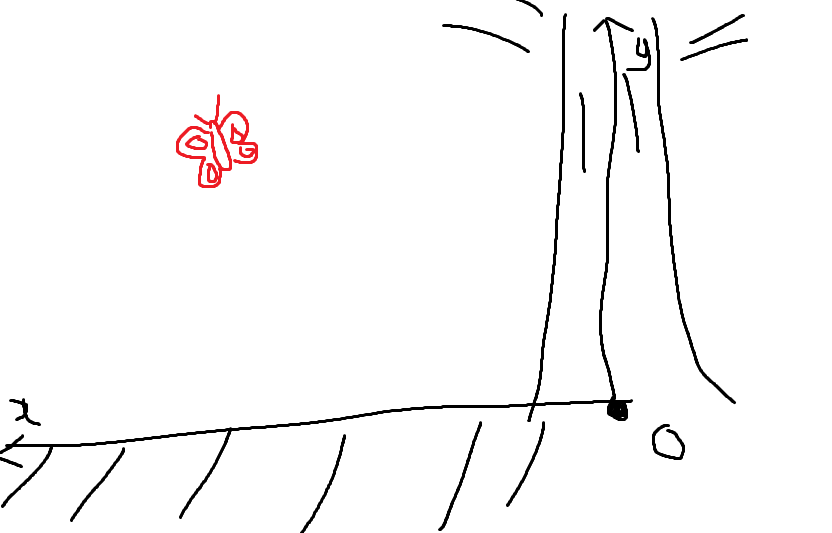
\includegraphics[scale=0.5]{2}
\end{center}
Now everything is so much easier now! You can just tell your friend "Hey, look at the \{middle of that tree; middle of the pavement\}" and you friend will instantly know where the butterfly is. In theory, you are saying a \textbf{coordinate} to your friend, the \textit{the middle of that tree} corresponds to the \textbf{x-coordinate} and the \textit{middle of the pavement} corresponds to the \textbf{y-coordinate} of that butterfly.\\
The Cartesian coordinate system is built on that premise, and though it may seem simple at first glance, this system is the preliminary to many other coordinate systems. 

\begin{center}
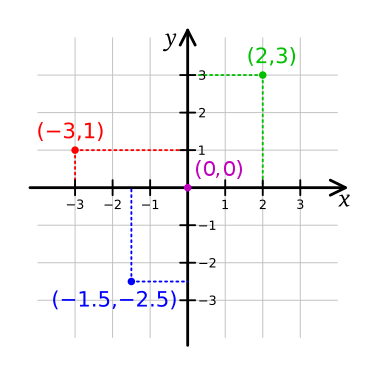
\includegraphics[scale=0.5]{3}
\end{center}

% %%%%%%%%%%%%%%%%%%%
\subsection*{P1.3}
% %%%%%%%%%%%%%%%%%%%
We call $x_\mathsf{new} = (1-\alpha)  x_\mathsf{old}+\alpha x_\mathsf{update}$ exponentially weighted because, simply, the weight for each older data of x decreases exponentially as we get newer data of x. To prove it, we change the notation of given function to: $$x_\mathsf{t} = (1-\alpha)  x_\mathsf{t-1}+\alpha x_\mathsf{update|t}$$
This recursive function can then be expanded to: $$x_\mathsf{t} = \alpha[x_\mathsf{t-1} +(1-\alpha)x_\mathsf{update|t-1} + (1-\alpha)^2x_\mathsf{update|t-2} + \ldots $$ 
$$ (1-\alpha)^kx_\mathsf{update|t-k}]+(1-\alpha)^{k+1}x_\mathsf{t-(k+1)}$$
wherein $x_\mathsf{t}$ is the Exponentially moving average at time t and $x_\mathsf{update|t}$ is the new value added to the data at time t. The $(1-\alpha)^k$ is an \textbf{exponential function}, discounting exponentially the value of older data as more data is added, hence the name exponentially weighted.

% %%%%%%%%%%%%%%%%%%%
\subsection*{P1.4}
% %%%%%%%%%%%%%%%%%%%
{\bfseries Prove that these are vector spaces:}
\subsubsection*{Cartesian product spaces $\mathbb{R}^n$}
Given $f$,$g \in \mathbb{R}^s$, with $s$ is a nonempty set and $f$,$g$ are $s$-tuples whose elements $\in \mathbb{R}$, and $c \in \mathbb{R}$, we have the following: 
$$f(s)+g(s)=\begin{bmatrix}
[x_{f1},x_{f2},x_{f3},\ldots]\\
[y_{f1},y_{f2},y_{f3},\ldots]\\
\vdots
\end{bmatrix} + 
\begin{bmatrix}
[x_{s1}, x_{s2}, x_{s3}\ldots]\\
[y_{s1}, y_{s2}, y_{s3}\ldots]\\
\vdots
\end{bmatrix}=
$$
$$
\begin{bmatrix}
[x_{s1} + x_{f1}, x_{s2} + x_{f2}, x_{s3} + x_{f3}\ldots]\\
[y_{s1} + y_{f1}, y_{s2} + y_{f2}, y_{s3} + y_{f3}\ldots]\\
\vdots
\end{bmatrix}$$
$$=(f+g)(s) \in \mathbb{R}^s$$ 
, $$cf(s)=c\begin{bmatrix}
[x_{f1},x_{f2},x_{f3},\ldots]\\
[y_{f1},y_{f2},y_{f3},\ldots]\\
\vdots
\end{bmatrix}
= \begin{bmatrix}
[cx_{f1},cx_{f2},cx_{f3},\ldots]\\
[cy_{f1},cy_{f2},cy_{f3},\ldots]\\
\vdots
\end{bmatrix}= (cf)(s) \in \mathbb{R}^\mathsf{s}$$
and
$$ (0+f)(s) = 0(s) + f(s) = f(s) $$
Therefore $\mathbb{R}^s$ is a vector space. Since $n = \{1,2,3,\ldots,n\}$, $\mathbb{R}^n$ is a vector space.

\subsubsection*{Matrices $\mathbb{R}^{m\times n}$ \& multi-dimensional arrays (data "tensors") $\mathbb{R}^{m\times n\times\dots\times q}$}
Since $\mathbb{R}^{n} \subseteq \mathbb{R}^{m \times n} \subseteq \mathbb{R}^{m\times n\times\dots\times q}$, and $\mathbb{R}^{n}$ is a vector space, we can logically conclude that $\mathbb{R}^{m \times n}$ and $\mathbb{R}^{m\times n\times\dots\times q}$ being vector spaces

\subsubsection*{$C[a, b]$ the set of all continuous functions on the closed interval $[a, b]$z}
Given the functions $f$,$g \in C[a, b]$, and $c \in \mathbb{R}$, we have the following:
$$f(x)+g(x)=(f+g)(x) \hspace{5mm}\forall x \in [a, b]$$
, $$ cf(x)= (cf)(x) \hspace{5mm}\forall x \in [a, b]  $$
and $$ (0 + f)(x) = 0(x) + f(x) = f(x)$$
By the algebra of continuous function, $f+g$ and $cf$ are continuous on $[a,b]$. Thus $C[a, b]$ is a vector space.

\subsubsection*{Space of all polynomials of one variable $x$ whose degree is at most $n$, $P_n(\mathbb{R}):=\{\sum_{i=0}^n a_i x^i\}$}
The space of $P_n(\mathbb{R}):=\{\sum_{i=0}^n a_i x^i\}$ is infinitely dimensional as $1,x,x^1,\ldots,x^n$ is linearly dependent for any n. With that said, given $f$,$g \in P_n(\mathbb{R})$ where $f(x) = \sum_{i=0}^n a_i x^i$, $g(x) = \sum_{i=0}^n b_i x^i$  and $c \in \mathbb{R}$, we have the following:
$$ f(x) + g(x) =  \sum_{i=0}^n a_i x^i +\sum_{i=0}^n b_i x^i = \sum_{i=0}^n (a_i+b_i) x^i = (f + g)x \hspace{5mm}\forall x \in [a, b]$$
and 
$$ cf(x) = c\sum_{i=0}^n a_i x^i = \sum_{i=0}^n ca_i x^i= (cf)(x) \hspace{5mm}\forall x \in [a, b]$$
Thus making the $P_n(\mathbb{R}):=\{\sum_{i=0}^n a_i x^i\}$ a vector space.
	
% %%%%%%%%%%%%%%%%%%%
\subsection*{P1.5}
% %%%%%%%%%%%%%%%%%%%
{\bfseries Prove that these are NOT vector spaces:}
\subsubsection*{The spaces of positive real axis}
Simply enough, the spaces of positive real axis does NOT contain a zero vector because this space defines to contain only positive real numbers ($>0$), thus making it not a vector space.

\subsubsection*{Unit vectors}
Given $\vec{u}^n$, a unit vector with a size of n, and $c \in \mathbb{R}$ we have the following:
$$c\vec{u}^n = c\begin{bmatrix}
1\\
0\\
\vdots 
\end{bmatrix} = \vec{u}^n = c\begin{bmatrix}
c\\
0\\
\vdots
\end{bmatrix} $$
The resulting vector is $\notin \vec{u}^n$, making unit vector $\vec{u}^n$ not a vector space. Applies to other types of unit vectors. Alternatively, we can say that unit vectors are not vector spaces because they does not contain a zero vector.

\subsubsection*{Latitude and longitude}
The problem with latitude and longitude is that it is bounded. The value of latitude is bounded between -90\textdegree and 90\textdegree, and the value of longitude is bounded between -180\textdegree and 180\textdegree. When we conduct addition or scalar multiplication on any $f = [langitude; longitude]$, $\exists langitude > 90\textdegree$ and/or $\exists longitude > 180\textdegree$, which invalidates the rules of the system, thus making latitude and longitude not vector space.

\subsubsection*{Monomials $\{x^k\}$}
The space of monomials does not form a vector space because it is not closed under addition or scalar multiplication. Given $f$,$g \in \{x^k\}$, we have the following:
$$ f(x) + g(y) = x^k + y^k \notin \{x^k\}$$
The same applies to scalar multiplication.


% %%%%%%%%%%%%%%%%%%%
\subsection*{P1.6} 
% %%%%%%%%%%%%%%%%%%%
{\bfseries A line through $v$ in direction of $u$: $L_1=\{w\in V: w = v+tu, ~\forall t\in\mathbb{R}, ~ u,v\in V\}$}\\
We can easily think of this line as a segment of a line bounded between point $v$ and point $u$ in the Cartesian coordinate system. The point $v$ here is the origin of the segment and $u$ is the direction of the segment, making this a vector. Now we extend this segment both side, and we have the desired line. How can this line be vector space $L_1=\{w\in V: w = v+tu, ~\forall t\in\mathbb{R}, ~ u,v\in V\}$?
Assume $v=(x_v, y_v)$, $u=(x_u, y_u)$ and $w=(x_w, y_w)$ as it does not break the generality of the given rules, we replaced it in the given equation $w = v+tu$:
$$ (x_w, y_w)= (x_v, y_v)+t(x_u, y_u) $$

\begin{equation*}
    \begin{cases}
              x_w= x_v+tx_u\\
              y_w= y_v+ty_u
         
          \end{cases}
\end{equation*}
The above equation forms a linear function, thus validating the vector space $L_1$ with $v,w,g$ as 2-dimension vectors. Applies with higher dimension of $v,w,g$.

\subsection*{P1.7} 

\subsection*{P1.8} 
{\bfseries A space $S$ is flat if any line between any 2 points of $S$ is contained in it $\Rightarrow$ All vector spaces are flat!}

If any line L between any 2 points of S is contained in it, and this $L$ is linear, then all addition and scalar multiplication will performed on $L$ will generate other linear $L$ that eventually covers all of the elements of said vector space, resulting in the "flatness" because of linear properties.


\subsection*{P1.12}
 {\bfseries What are the standard basis (and associated coordinate vectors) of $\mathbb{R}^d$, $\mathbb{R}^{m\times n}$, and $P_n(\mathbb{R})$?}\\
The standard basis of $\mathbb{R}^d$ is $E = \{(x_1, x_2, \ldots, x_d),$ where $x_j=1$ and the rest of $x = 0$ as $j$ approaches d from 1$\}$\\
The standard basis of $\mathbb{R}^{m \times n}$ is $E = 
\{\begin{bmatrix}
x_{1|1} & x_{1|2} &\ldots & x_{1|i}\\
x_{2|1} & x_{1|2} &\ldots & x_{2|i}\\
\vdots	&		&	\ddots\\
x_{i|1} & x_{i|2} &\ldots & x_{i|j}
\end{bmatrix},$ where $x_{i|j}=1$ and the rest of $x = 0$ as $i,j$ approaches $m,n$ from 1$\}$\\
The standard basis of $P_n(\mathbb{R})$ is $ E = \{1,x,x^2,x^3,...,x^n\}$.

\subsection*{P1.13}
{\bfseries So what does “linear” really mean, in linear combination?}\\
So what I think of linear is like how an $x$ would correspond to only one $y$ in a "straight line". That is, with only one feature ($x$), we can somewhat know how that certain thing ($y$, or output) would look like. With linear combination, we can have multiple features ($x$) being combined together to output this thing ($y$), and we would increase more of the knowledge of $y$, and the way we can discriminate between different $y$. Linear combination is a compact \textit{machine} where instead of having to store multiple $y$ with its multiple features ($x$), we only need this linear combination that can let us discriminate that output $y$.

\subsection*{P1.13}
{\bfseries Consider vector space $\mathbb{R}^3$. Let's choose a basis $B$ with 3 vectors:
$$e_1=(\frac{1}{\sqrt{2}}, \frac{1}{\sqrt{2}},0), e_2=(-\frac{1}{\sqrt{2}}, \frac{1}{\sqrt{2}},0), e_3=(0,0,1)$$
What are the coordinates in this basis $B$ of a vector in $\mathbb{R}^3$?}
$$v=a_1(\frac{1}{\sqrt{2}}, \frac{1}{\sqrt{2}},0)+a_2(-\frac{1}{\sqrt{2}}, \frac{1}{\sqrt{2}},0)+a_3(0,0,1)$$
or
$$v=(\frac{a_1}{\sqrt{2}}-\frac{a_2}{\sqrt{2}},\frac{a_1}{\sqrt{2}}+\frac{a_2}{\sqrt{2}},a_3)$$
% %%%%%%%%%%%%%%%%%%%
\section*{Section E}
% %%%%%%%%%%%%%%%%%%%
\subsection*{E1.1}
Assume $v \in span(S)$, then we have the following:
$$ \begin{bmatrix}
9\\
16\\
29
\end{bmatrix}= a_1\begin{bmatrix}
1\\
2\\
3
\end{bmatrix} + a_2\begin{bmatrix}
2\\
4\\
6
\end{bmatrix} + a_3\begin{bmatrix}
1\\
1\\
4
\end{bmatrix}$$


Equals to\\
\begin{equation*}
    \begin{cases}
              9= a_1+2a_2+a_3\\
              16= 2a_1+4a_2+a_3\\
         	  29= 3a_1+6a_2+4a_3
          \end{cases}
\end{equation*}
\begin{equation*}
    \begin{cases}
              7 = a_1+2a_2\\
     
         	  29= 3(a_1+2a_2)+4a_3
          \end{cases}
\end{equation*}

\begin{equation*}
    \begin{cases}
              7 -a_2 = a_1\\
     
         	  2= a_3
          \end{cases}
\end{equation*}

We then have: 
$$ v
= (7 -a_2)\begin{bmatrix}
1\\
2\\
3
\end{bmatrix} + a_2\begin{bmatrix}
2\\
4\\
6
\end{bmatrix} + 2\begin{bmatrix}
1\\
1\\
4
\end{bmatrix}$$ 
For all $a_2 \in \mathbb{R}$, we can conclude by definition that $v \in span(s)$

\subsection*{E1.2}
We have $S=\{v_1,\ldots,v_n\} \in V$ and $span(S) = \{v = a_1v_1+\ldots+a_nv_n, a_1,\ldots, a_n \in \mathbb{R}\}$. $span(S)$ is obviously the subspace of $V$ as $V$ closes under vector addition and scalar multiplication, and it is also obvious that $S$ is a subset of $span(S)$ because $span(S)$ is the set containing all the possible linear combinations of $S$. 	\\
Now, suppose that $W$ contains $S$, and since $W$ itself is a vector space, then it also contains every linear combinations of $S$ ($W$ is closed under vector addition and scalar multiplication), which happens to be $span(S)$. We can then conclude that $W$ has to be as large as $span(S)$, thus making $span(S)$ the smallest subspace that contains $S$.

\subsection*{E1.3}
A vector space $V$ is said to be linearly dependent if $$\sum_{i=0}^n a_i v_i=0$$ where in $a_1, a_2,\ldots,a_i$ are scalars, not all zero, and $v_1,v_2,\ldots,v_i \in S$. Now we can conclude that ${\varnothing}$ is linearly independent, because simply it does not have any collection of $a$ that contains at least 1 non-zero scalars (it is empty in itself, so every scalars in it is automatically $0$).

\subsection*{E1.4}
In the case of $\{0\}$, $\exists a \neq 0$ such that $a\vec{0}=\vec{0}$. Therefore it is linearly dependent by definition. The same applies to any vector space that contains
$\vec{0}$, as in the collection of scalars $a_1, a_2,\ldots,a_i$ of said vector space $S=\{v_1,v_2,\ldots,v_n\}$, $\exists a_1 \neq 0, a_2,...,a_n=0$, which makes $a_10 + a_2v_2 +\ldots + a_nv_n = 0$ (we can safely assume that $v_1=0$ as it does not break the generality of the statement).

\subsection{E1.5}
Assume for contradition that there exists a $\{b_1, \dots, b_n\}$ $\exists i \in \{1,\dots,n\} \text{ s.t. } b_i \neq a_i$ $v = \sum_{i=1}^n b_i v_i$ beside $\{a_1, \dots, a_n\}$ , $v = \sum_{i=1}^n a_i v_i$. Then we will have the following: 
$$\sum_{i=1}^n b_i v_i=v=\sum_{i=1}^n a_i v_i$$
Equals to:
$$\sum_{i=1}^n (a_i- b_i) v_i=0$$
Thus
$$a_i- b_i = 0 \Leftrightarrow a_i = b_1$$
contradicting the $b_i \neq a_i$ notion. We then can conclude that the collection $\{a_1, \dots, a_n\}$ , $v = \sum_{i=1}^n a_i v_i$ is unique.


\newpage 






\end{document}
